\clearpage

\section{Neumayer III \& AWIPEV}
\label{Sec:LocalDTRTrend}

In the following section, data meterological data from the stations "Neumayer III" and "AWIPEV" is analysed.

% The diurnal temperature trend at AWIPEV, a station in the northern hemisphere near Spitsbergen, shows a decreasing trend. This is in accordance with the observations made in \cref*{sec:DTRmonth}.
% The diurnal cycle of the sun is a subordinate factor in the DTR. In a Fourrier analysis of the temperature data, the diurnal cycle of the sun caused a frequency of 24 hours a signal 
% with the amplitude of 0.3 °C. This account for less than 10 \% of the DTR. The most important contributions to DTR are fluctuations on a shorter time scale and large temperature
% changes on a a multi-day time scale.
\subsection*{Arctic}

The diurnal temperature trend observed at AWIPEV, a research station situated in the northern hemisphere near Spitsbergen, exhibits a declining pattern as shown in \cref{fig:AWIPEVcomparison}. This observation aligns with the findings presented in \cref*{sec:DTRmonth}.
\begin{figure}[ht]
    \centering

    \begin{subfigure}[t]{0.48\textwidth}
        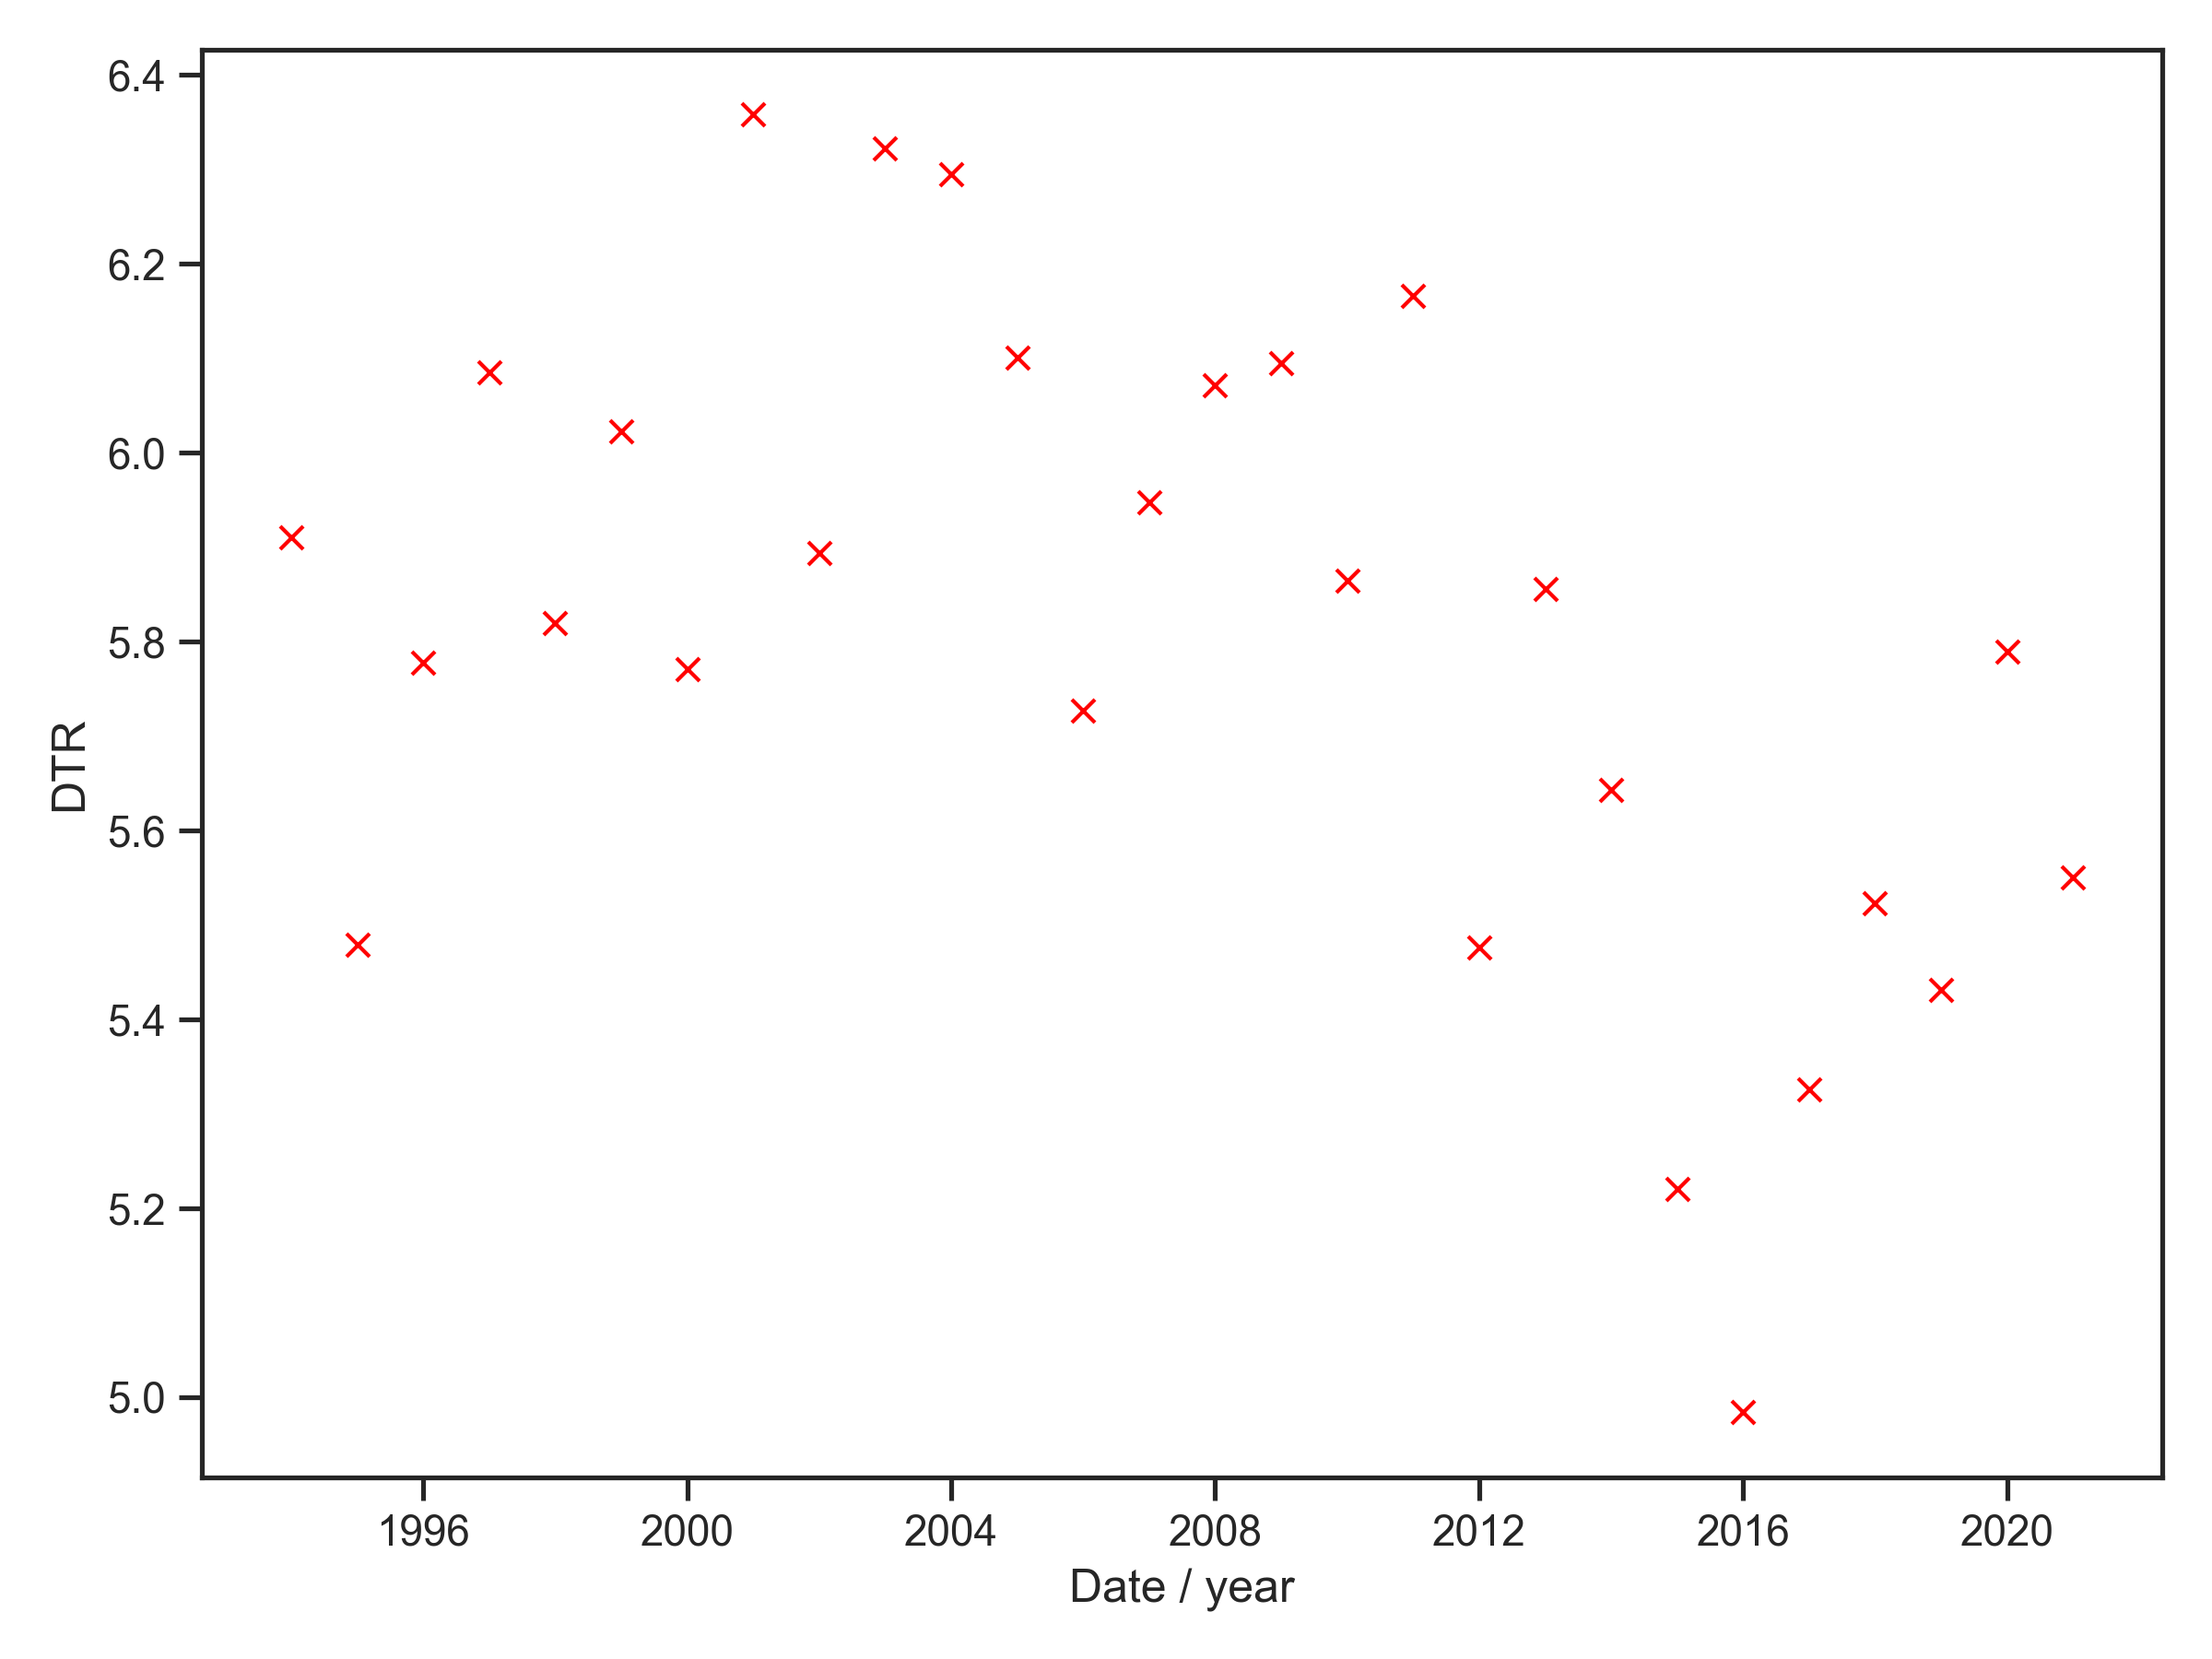
\includegraphics[width=\linewidth]{C:/Users/leonh/Desktop/Praktikum_AWI/Spitzbergen/SB_DTR_year.png}
        \caption{Yearly mean diurnal temperature range at meteorological station AWIPEV near Spitsbergen.}
        \label{fig:DTRyearAWIPEV}
    \end{subfigure}
    \hfill
    \begin{subfigure}[t]{0.48\textwidth}
        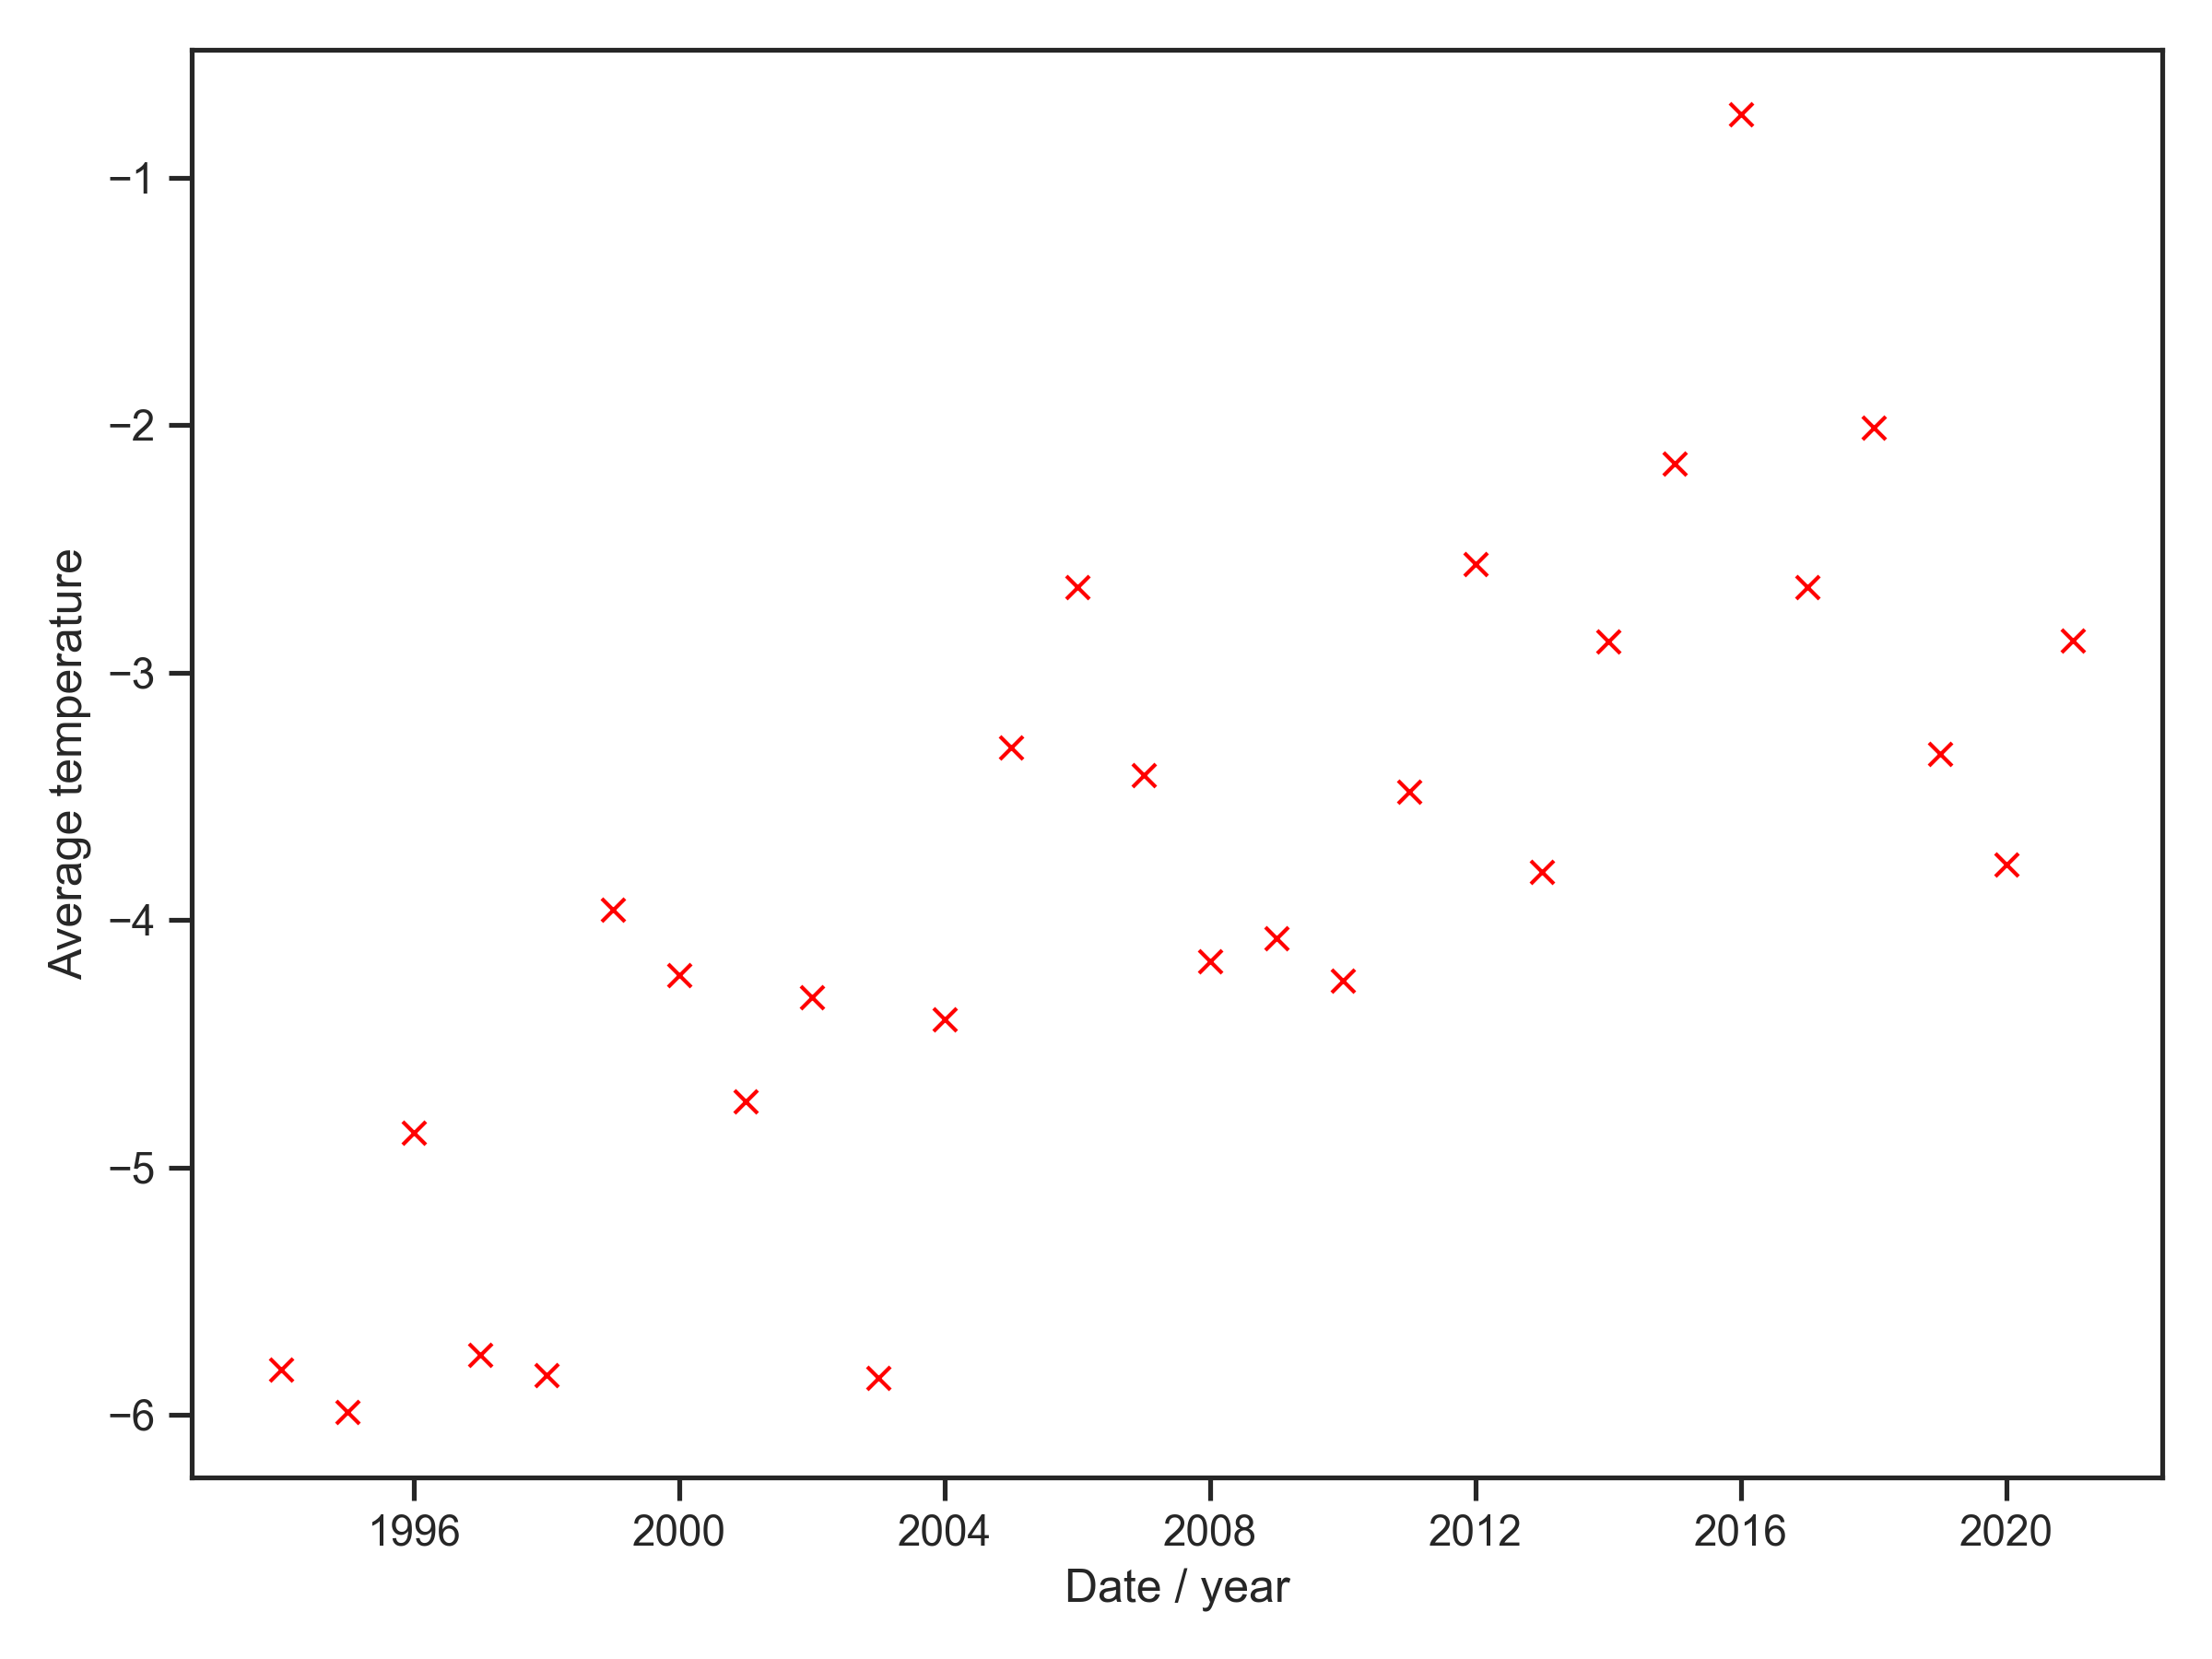
\includegraphics[width=\linewidth]{C:/Users/leonh/Desktop/Praktikum_AWI/Spitzbergen/SB_Date_T2Avg.png}
        \caption{Yearly mean temperature at meteorological station AWIPEV near Spitsbergen.}
        \label{fig:TAvgyearAWIPEV}
    \end{subfigure}
    \caption{Comparison of temperature data at AWIPEV station.}
    \label{fig:AWIPEVcomparison}
\end{figure}

% The diurnal cycle of solar radiation, although at mid-latitudes a significant factor, plays a subsidiary role in influencing the Diurnal Temperature Range.
% In a Fourier analysis of the temperature dataset, the diurnal solar cycle produces a signal with a 24-hour frequency and an amplitude of below 0.3 °C.
% However, this contribution accounts for less than 5\% of the overall DTR. The most substantial contributions to DTR are attributable to shorter-term fluctuations and
% significant temperature variations occurring over multiple days.
Although the diurnal cycle of solar radiation plays a subsidiary role in influencing the Diurnal Temperature Range, it is a significant factor at mid-latitudes.
In a Fourier analysis of the temperature dataset, the diurnal solar cycle produces a signal with a 24-hour frequency and an amplitude of less than 0.3 °C. However, this contribution makes up less than 5\% of the overall DTR. Shorter-term fluctuations and significant temperature variations occurring over multiple days are responsible for the most substantial contributions to DTR.

Examining the correlation between the different recorded variables, we can observe a strong connection between the average temperature and the DTR range.

\begin{figure}[ht]
    \centering
    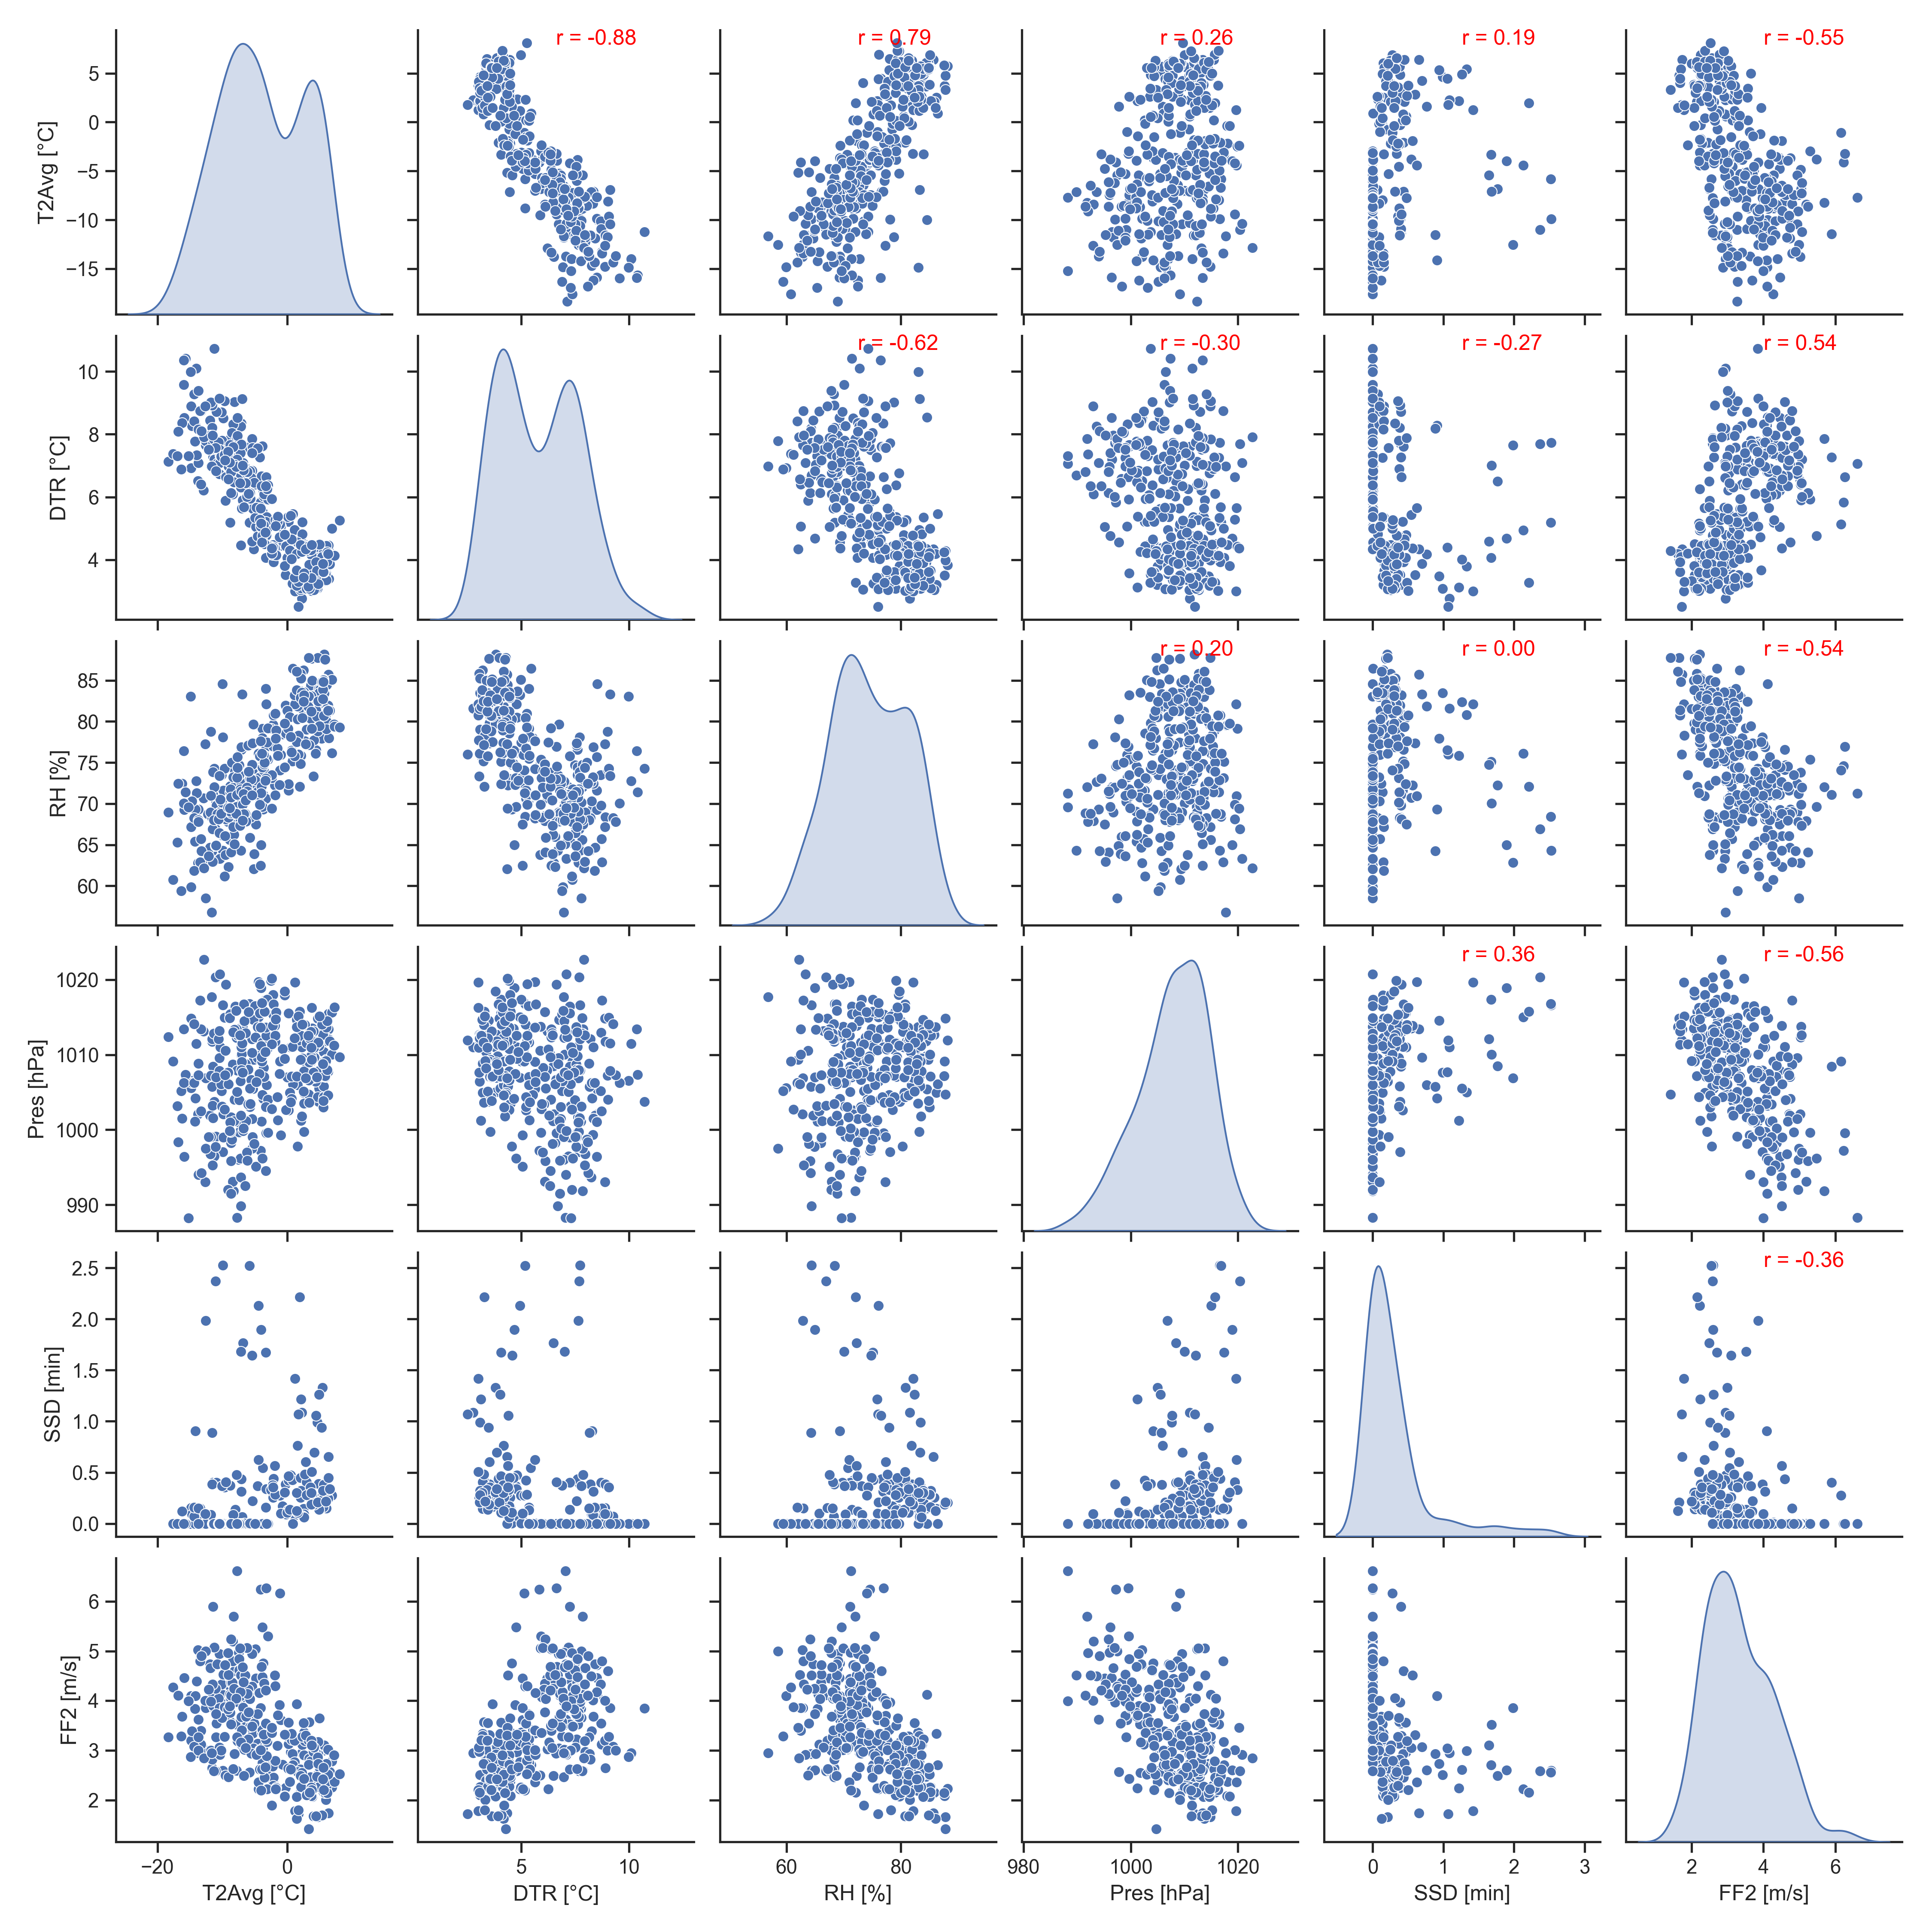
\includegraphics[width = \textwidth]{C:/Users/leonh/Desktop/Praktikum_AWI/Spitzbergen/SB_correlations_month.png}
    \caption{Correlation between average temperature, diurnal temperature range, relative humidity, air pressure, sunshine duration and wind speed.}
    \label{fi:correlationMonth_SB}
\end{figure}

% When plotting the DTR against the average temperature (see \cref{fig:SB_DTR_Month_scatterd}), there seem to be two regimes. One with falling DTR below approximately 
% \SI{0}{\celsius}. For average temperatures above the freezing point the DTR grows again. 
When plotting the DTR against the average temperature (refer to Figure \ref{fig:SB_DTR_Month_scatterd}), two distinct regimes become apparent. In the first regime, the DTR decreases with increasing temperatures for average temperatures up to \SI{2}{\celsius}. However, for average temperatures above this limit, the DTR starts to increase again.

\begin{figure}[ht]
    \centering
    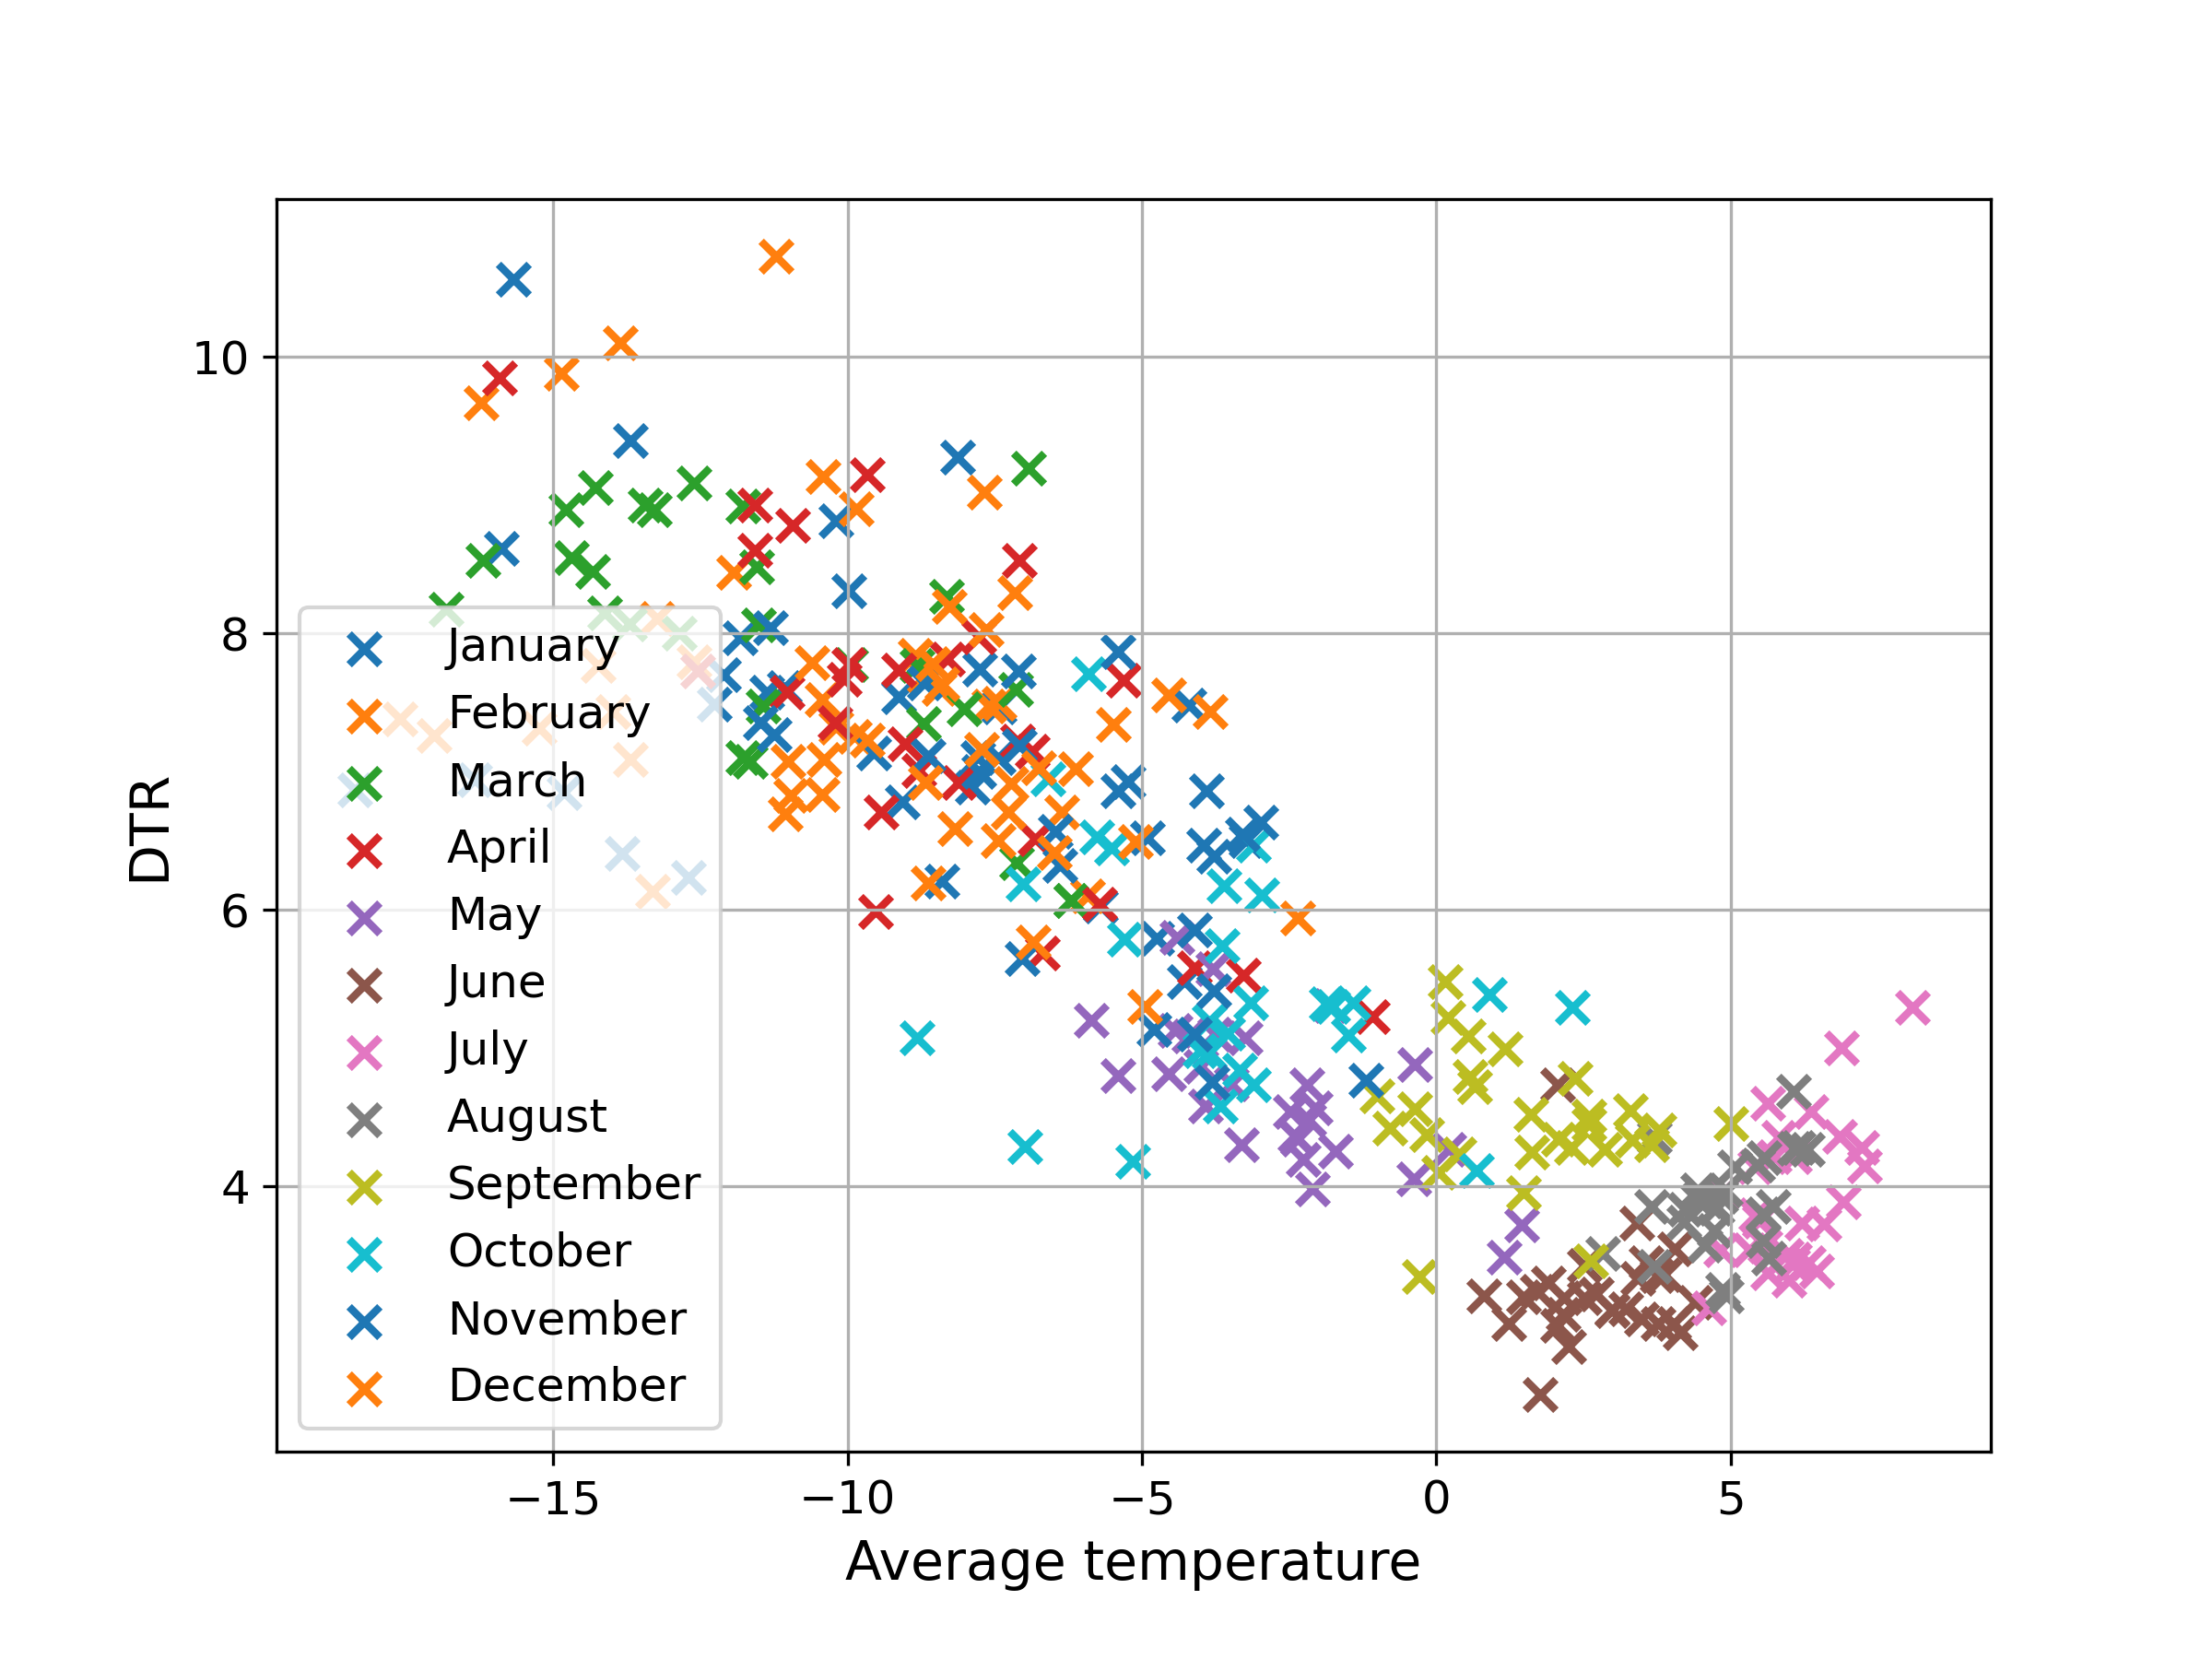
\includegraphics[width = \textwidth]{C:/Users/leonh/Desktop/Praktikum_AWI/Spitzbergen/SB_DTR_T2Avg.png}
    \caption{Comparing Monthly Diurnal Temperature Ranges with Average Monthly Temperatures at Arctic Meteorological Station \textit{AWIPEV} from 1983 to 2022}
    \label{fig:SB_DTR_Month_scatterd}
\end{figure}

% The minimal diurnal temperature difference near the freezing point reveals one dominate
% phenomena. At \SI{0}{\celsius}, the transition of ice from solid to liquid occurs. During this transition, latent heat is absorbed, exerting a cooling effect on the maximum daily temperature. Conversely, temperatures below the freezing point are increased as long there is water in the fluid state present as it releases the latent heat while freezing. IF freezing were the dominant process we would expect the lowest effect at \SI{0}{\celsius}.
% The shift in the DTR minimum can be attributed to the difference between ground temperatures and temperatures at 2 meters above the ground.

Near the freezing point, a minimal diurnal temperature difference reveals one dominant phenomenon: the transition of ice from a solid to a liquid state at \SI{0}{\celsius}. During this transition, latent heat is absorbed, exerting a cooling effect on the maximum daily temperature. Conversely, temperatures below the freezing point increase as long as there is water in the fluid state present, as it releases latent heat while freezing. If freezing were the dominant process and the measurement was ideal, we would expect the lowest effect at \SI{0}{\celsius}.
The shift in the minimum diurnal temperature range could be caused to the disparity between ground temperatures and air temperatures at 2 meters above the ground.

As temperatures rise above freezing point, the snow cover will shrink. This reduction diminishes the insulating properties of snow, rendering the environment more susceptible to external influences. This change in insulation could potentially have a significant impact on diurnal temperature range.


% A significant external influence is an enhanced heat transport mechanism. Altered thermal dynamics, coupled with reduced snow cover, facilitate increased heat exchange within the environment. Consequently, this influences and modulates the daily temperature fluctuation, contributing to the complexity of temperature variations near the freezing point.

\subsection*{Antarctica -- Georg von Neumayer III}

% In the following, the data from Antarctica are analysed in the same way as the AWIPEV data as shown in \cref{fig:GVN_DTR_Month_scatterd}.
% The trends observed at AWIPEV can also be noticed here. However, only the regime for temperatures below 0 degrees Celsius is observable.
In the following section, we analyze the data from Antarctica using the same approach as demonstrated with the AWIPEV data, as illustrated in Figure \ref{fig:GVN_DTR_Month_scatterd}. The trends observed at AWIPEV are also discernible here. However, it's important to note that we can only observe trends in temperatures below 0 degrees Celsius.

\begin{figure}[h!]
    \centering
    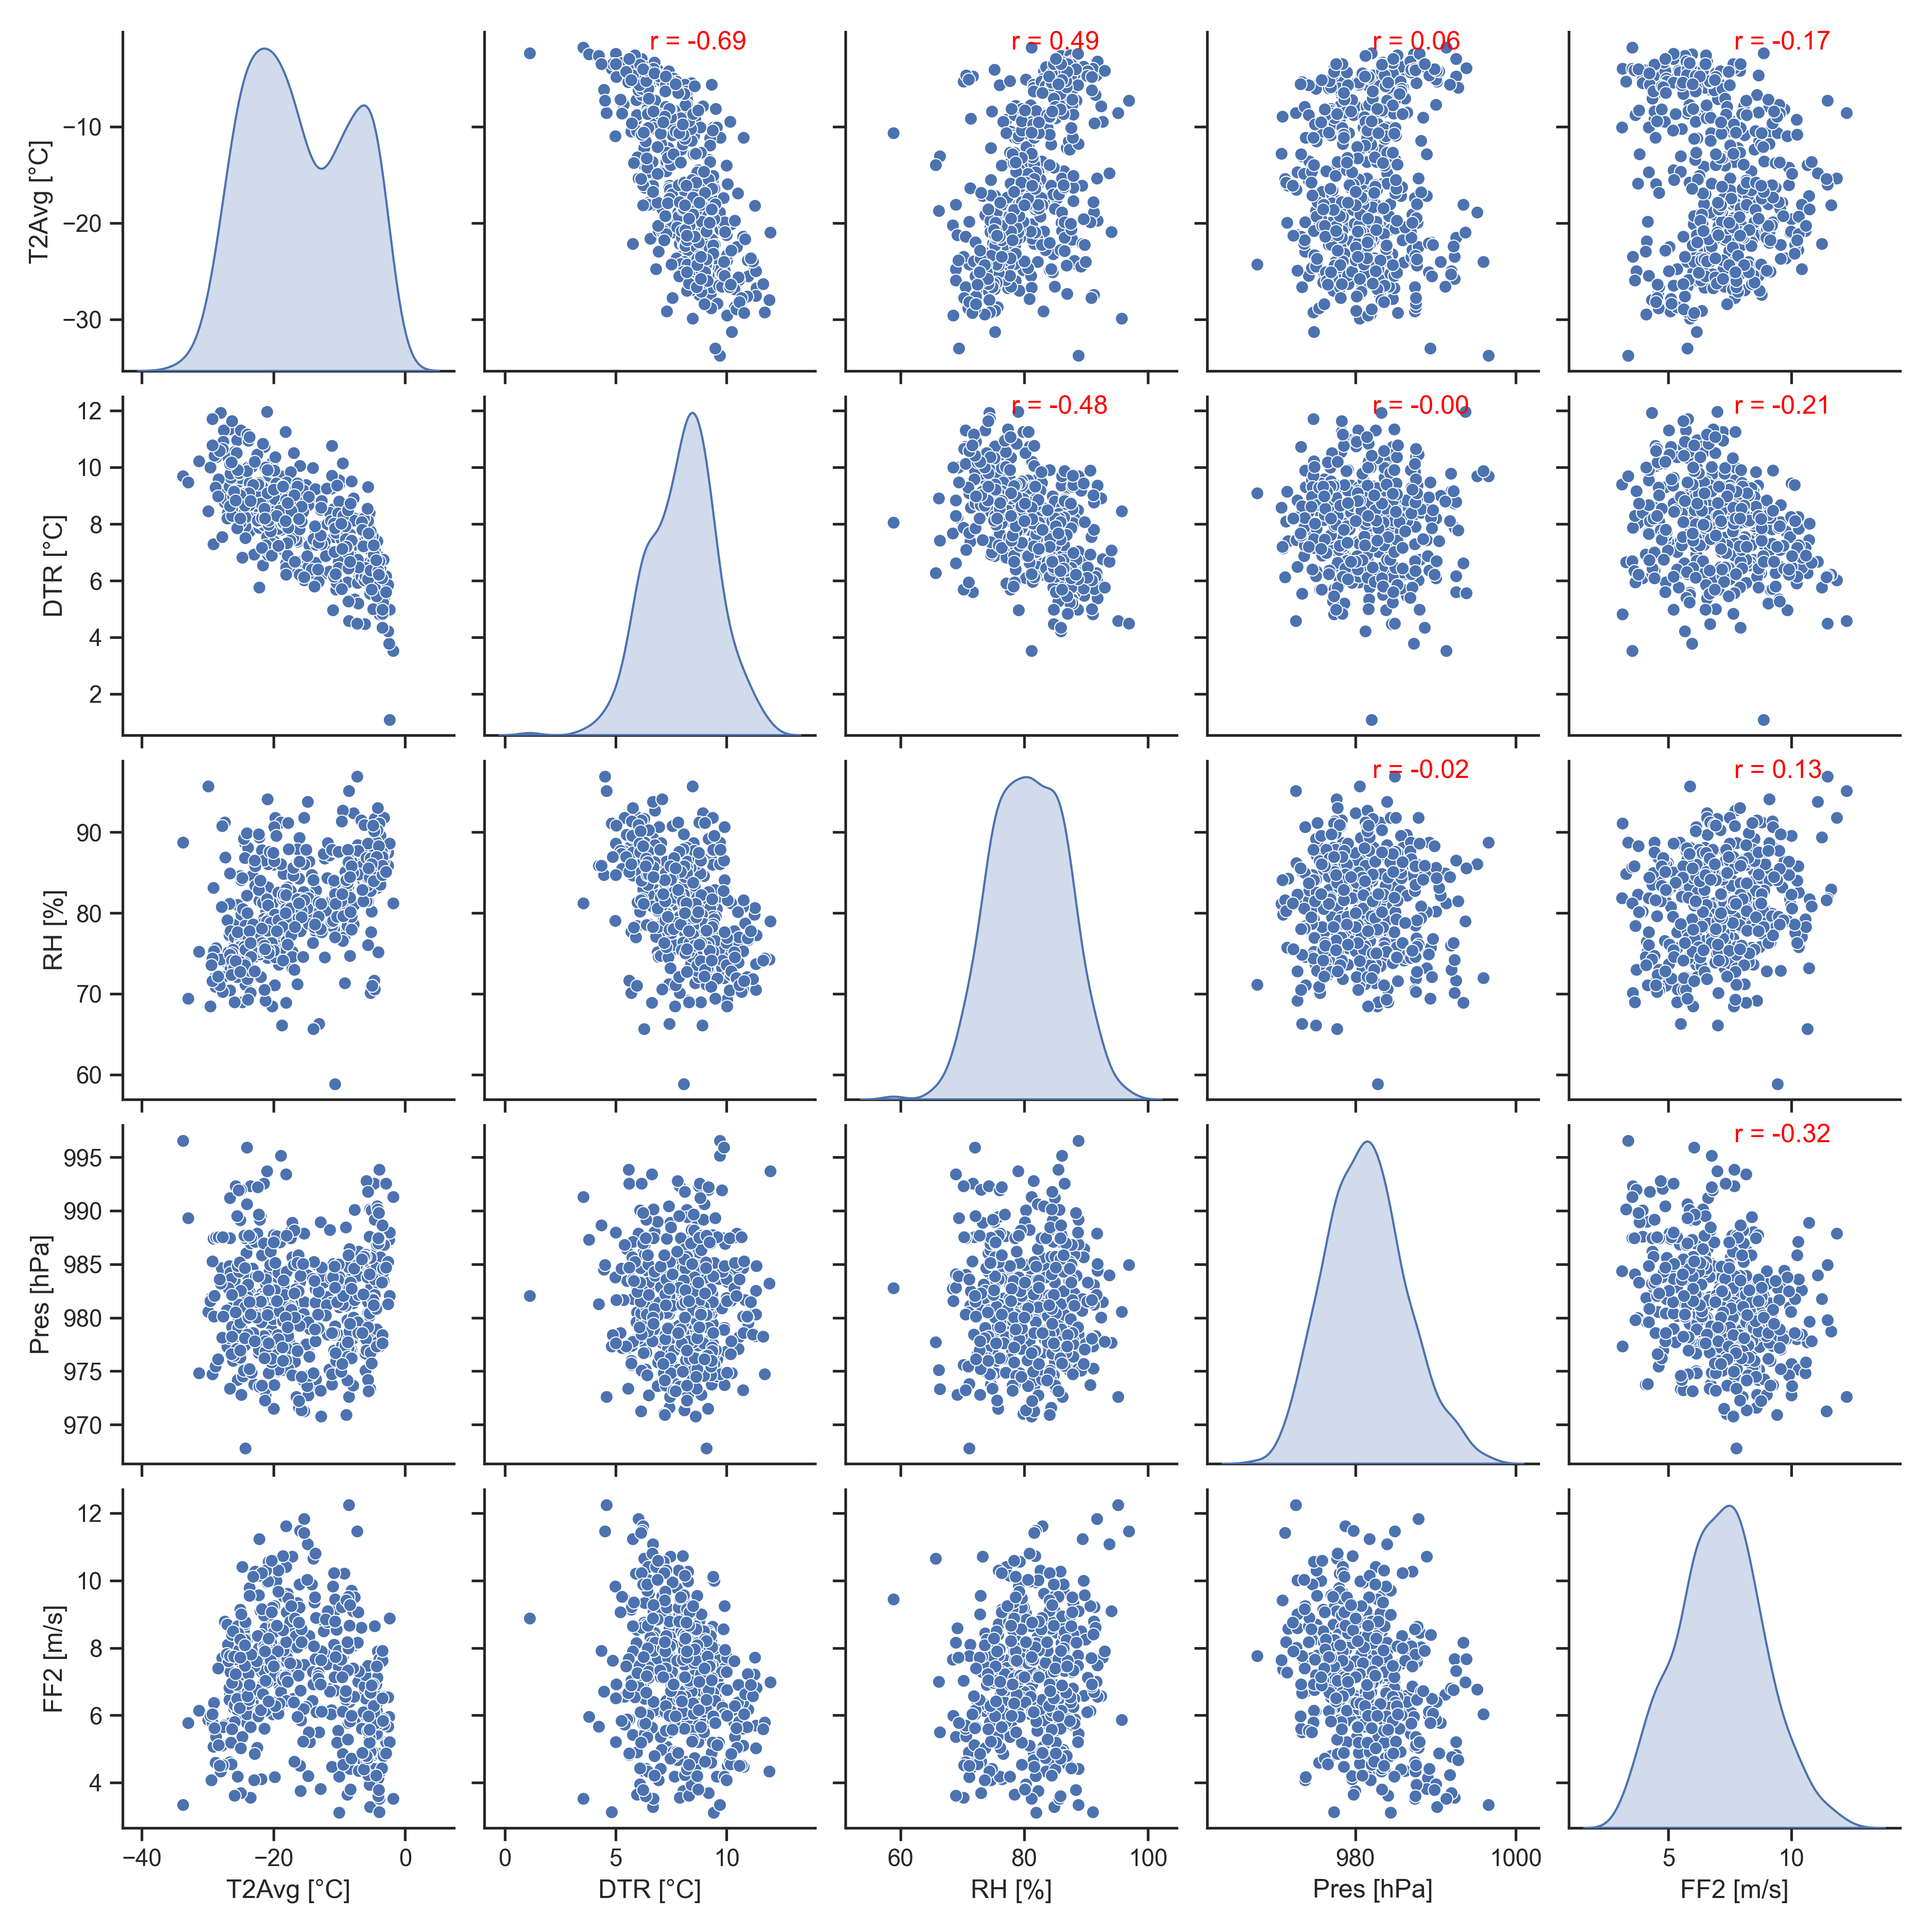
\includegraphics[width = \textwidth]{C:/Users/leonh/Desktop/Praktikum_AWI/GVN/GVN_correlation_month.png}
    \caption{Comparing Monthly Diurnal Temperature Ranges with Average Monthly Temperatures at Antarctica's Neumayer Meteorological Station from 1983 to 2022}
    \label{fig:GVN_DTR_Month_scatterd}
\end{figure}


% The strongest correlation observed at Neumayer is between the average temperature and the diurnal temperature range (DTR), which is similar to the observation at AWIPEV.
% The correlation becomes stronger when observing the monthly means compared to the daily means (see \cref{fig:SB_DTR_days_scatterd,fig:GVN_DTR_days_scatterd}).
% This stronger correlation when calculating the monthly mean could be explained by a delay of the effect.
% An example of such an delay could be caused by a lower heat transport in the laminar boundary layer. This delays the warming of the ice until the melting point.

The Neumayer station exhibits a notably robust correlation between average temperature and diurnal temperature range, a pattern that resembles observations at AWIPEV. This correlation strengthens when analyzing monthly means as opposed to daily averages, as depicted in \cref{fig:SB_DTR_days_scatterd,fig:GVN_DTR_days_scatterd}.

The heightened correlation when considering monthly means may be attributed to a delayed effect. One plausible explanation for this delay could be the reduced heat transport within the laminar boundary layer. This delay results in a postponed increase in ground temperature leading to delayed melting. Another explanation could be the melting of snow, which insulates the soil.

\section{Comparing trends in the Arctic and Antarctica}

% The declining trends in DTR between \SI{-20}{\celsius} and \SI{0}{\celsius} mean temperature are comparable at Neumayer and AWIPEV. The signal from Neumayer is noisy in the
% for temperatures close to \SI{0}{\celsius}.The trend of decreasing Diurnal Temperature Range initiates when the extremities of the DTR distribution reach freezing point, under the assumption that the DTR distribution is symmetrically centered around the mean temperature.
The declining trends in DTR between \SI{-20}{\degreeCelsius} and \SI{0}{\degreeCelsius} mean temperature are comparable at Neumayer and AWIPEV. However, the signal from Neumayer exhibits noise, particularly when temperatures are near \SI{0}{\degreeCelsius}. The trend of decreasing Diurnal Temperature Range begins when the outermost values of the DTR distribution approach the freezing point, assuming that the DTR distribution is symmetrically centered around the mean temperature.
\begin{figure}[ht]
    \centering
    \begin{subfigure}[t]{0.49\textwidth}
        \centering
        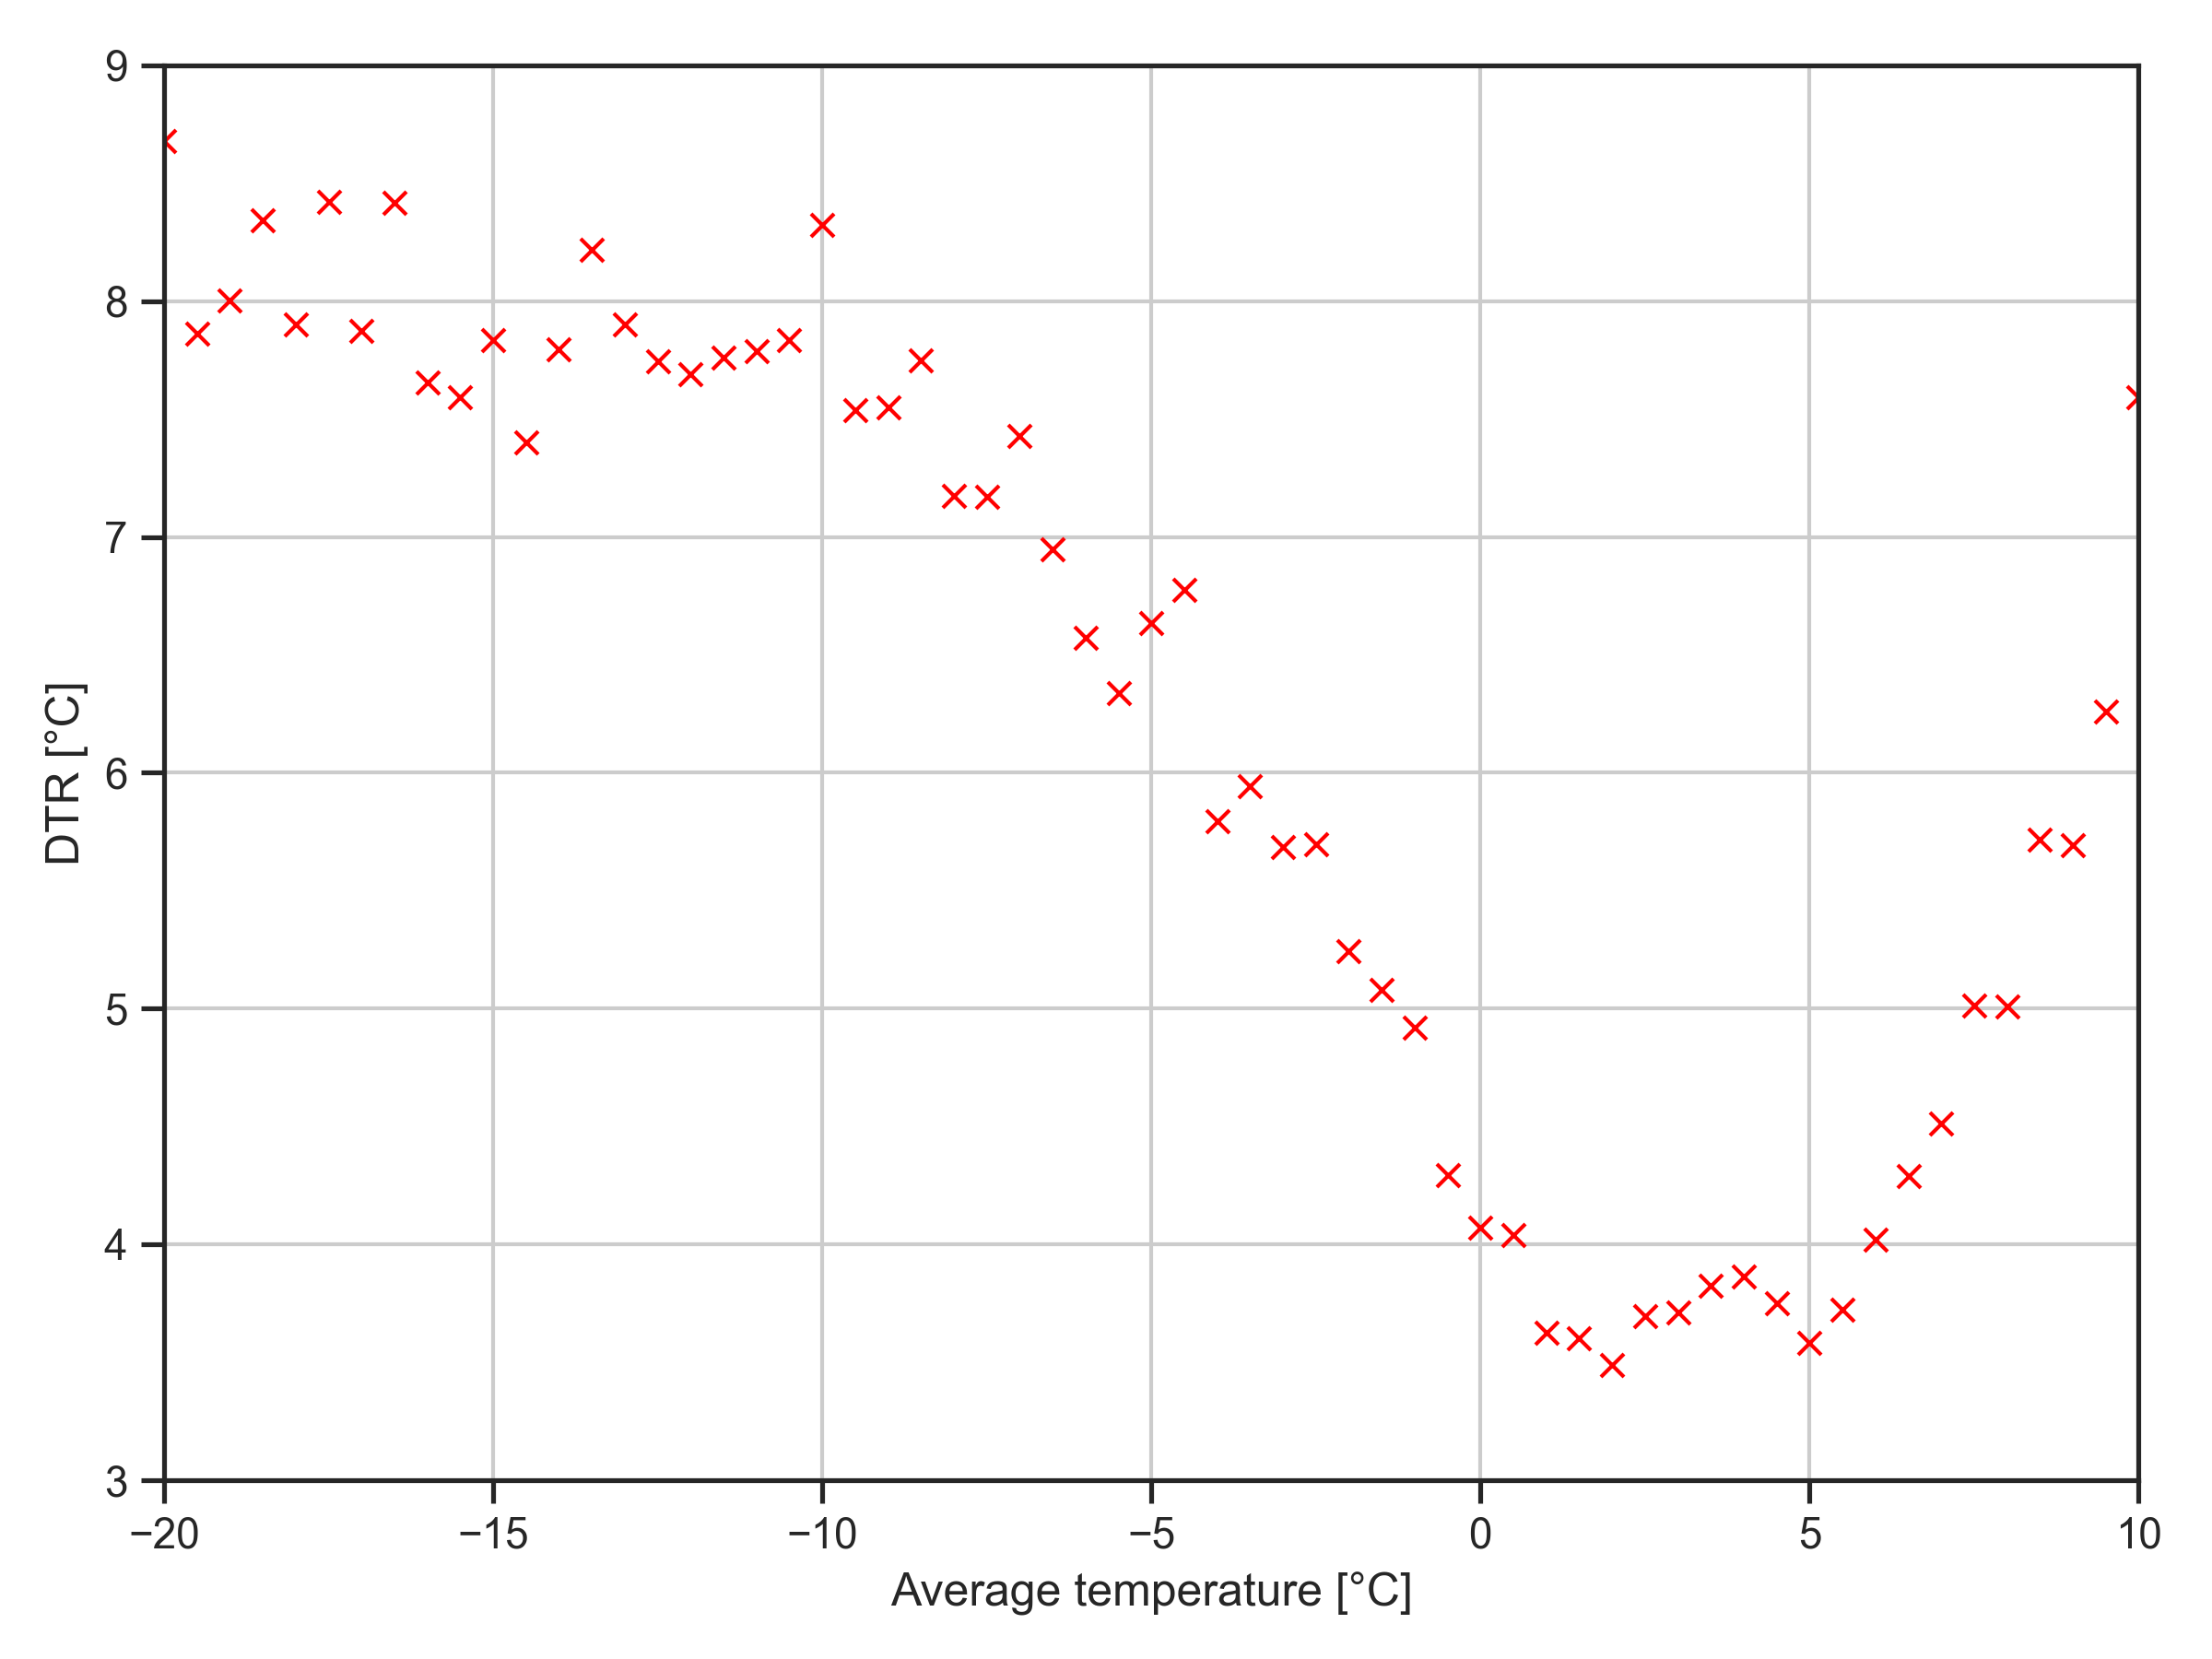
\includegraphics[width = \textwidth]{C:/Users/leonh/Desktop/Praktikum_AWI/Spitzbergen/SB_DTR_binning.png}
        \caption{AWIPEV}
        \label{subfig:DTRbinningAWIPEV}
    \end{subfigure}
    \hfil
    \begin{subfigure}[t]{0.49\textwidth}
        \centering
        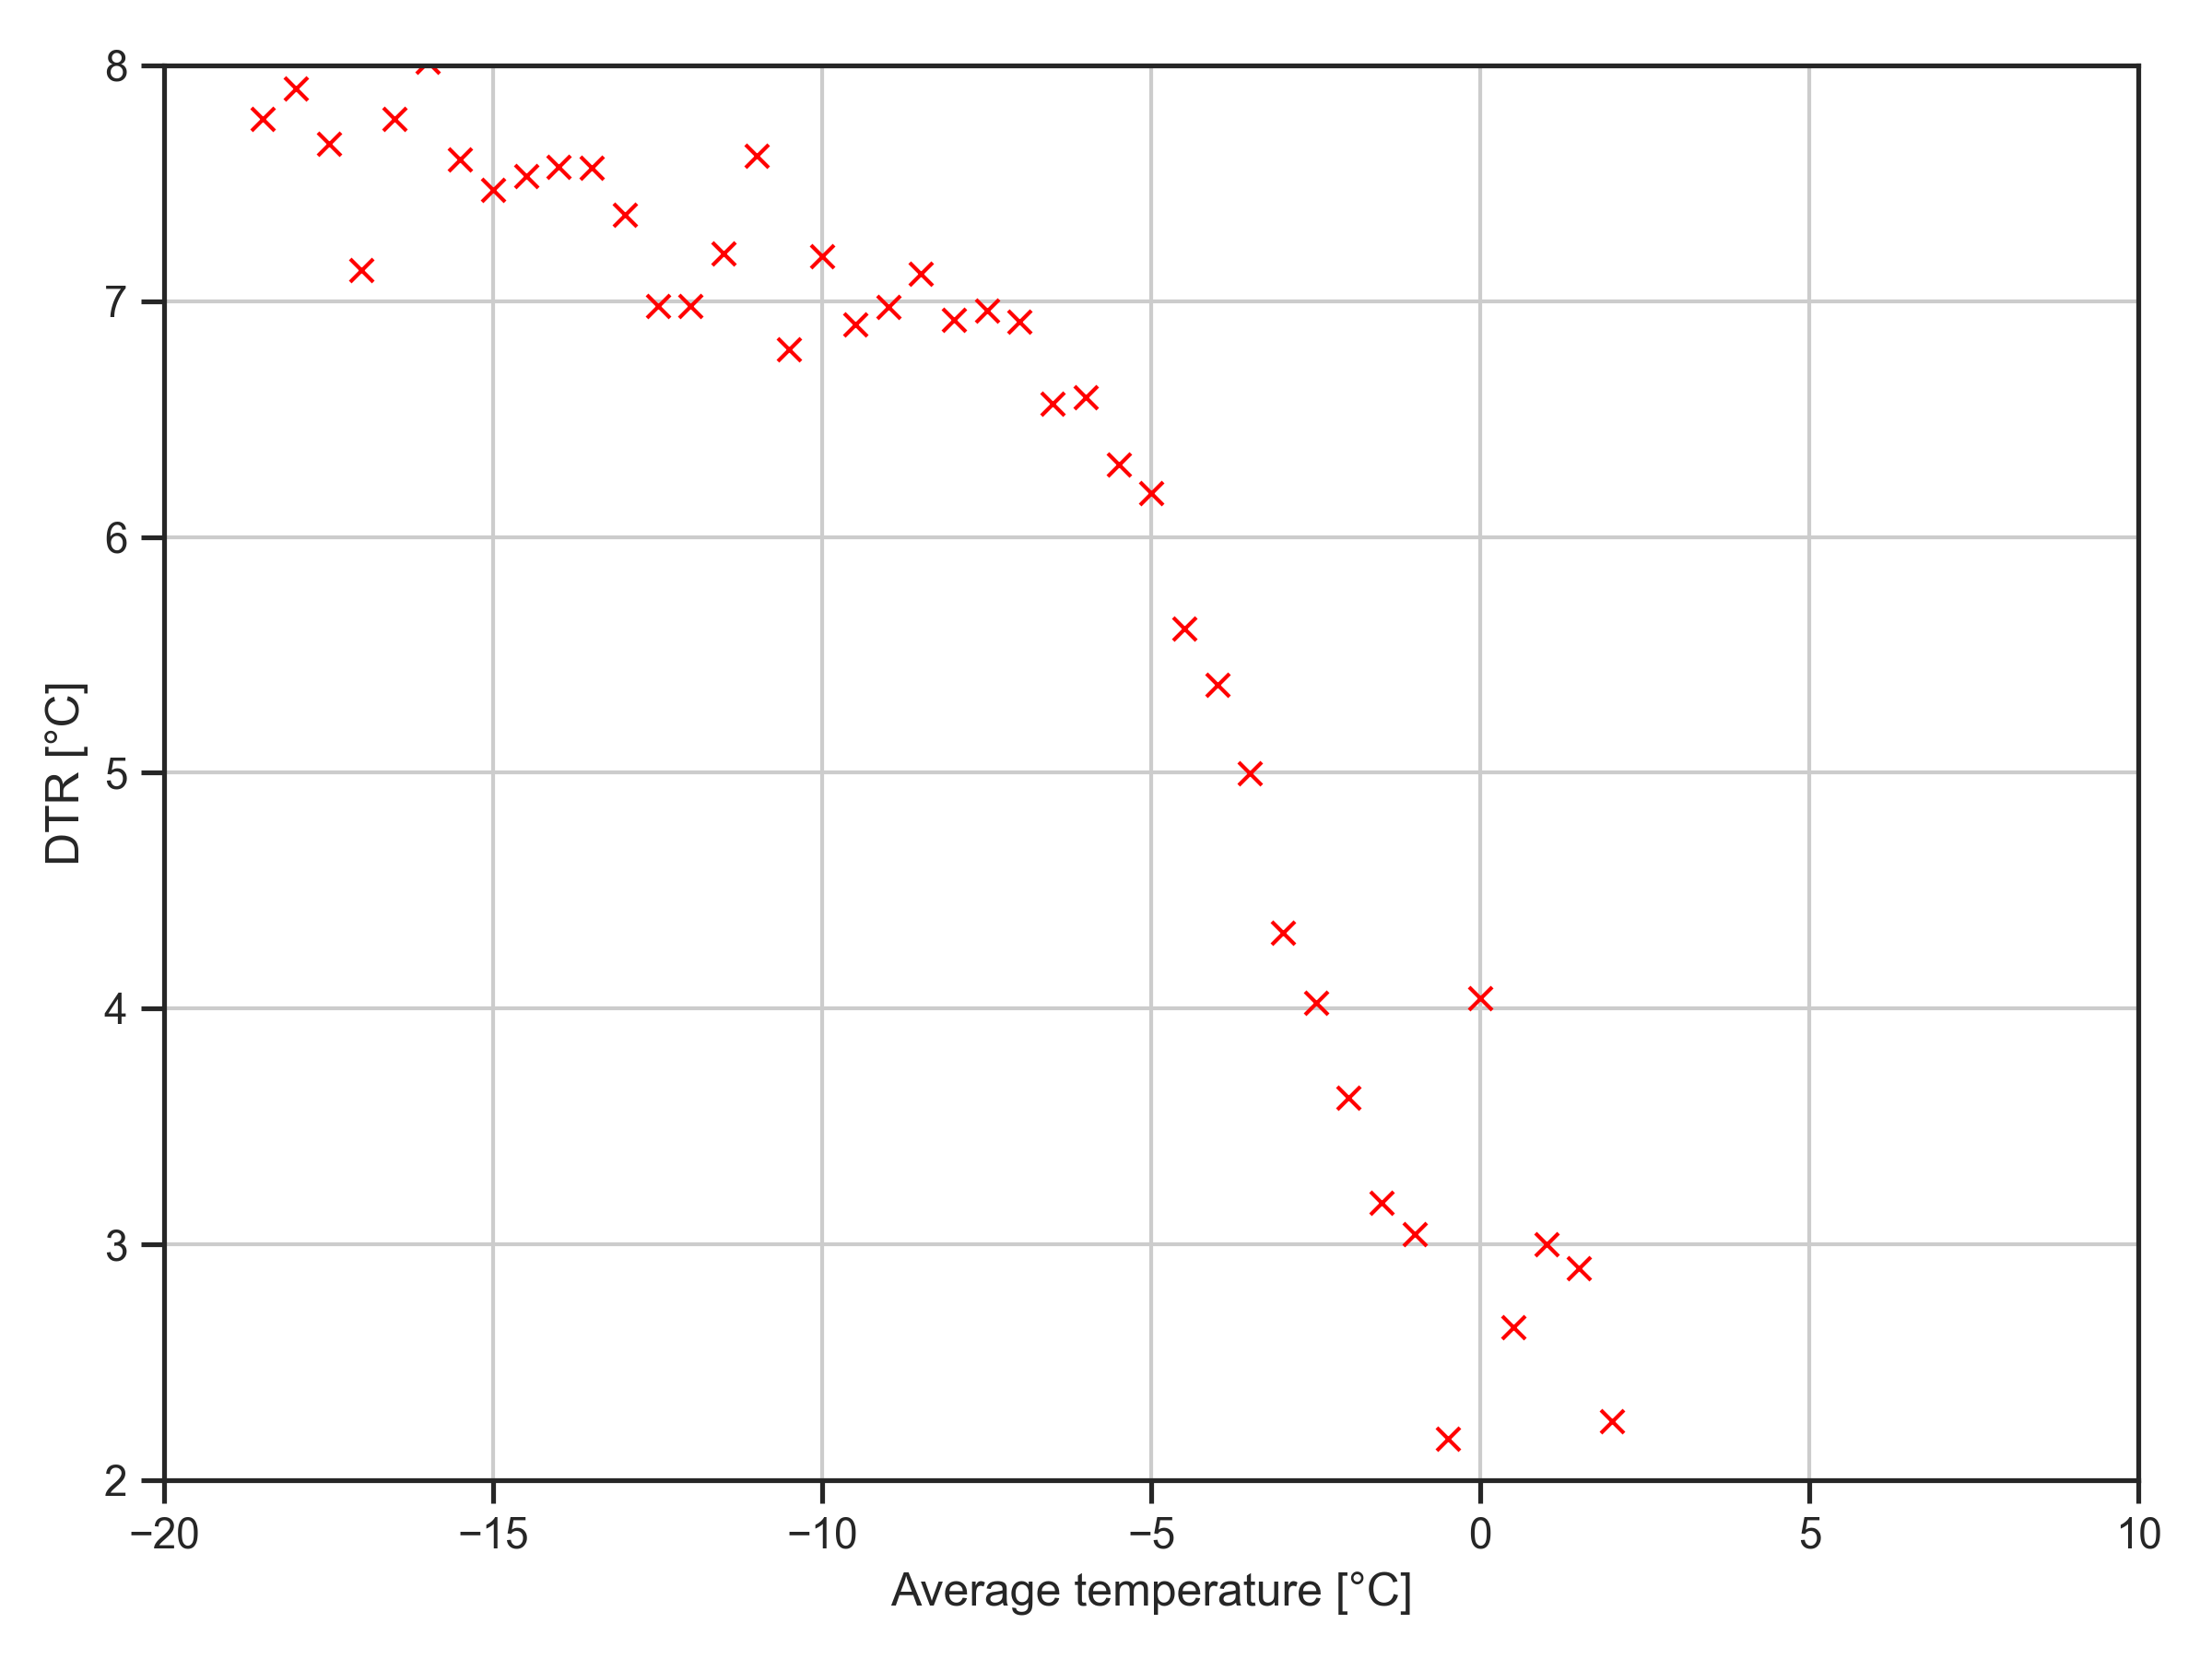
\includegraphics[width = \textwidth]{C:/Users/leonh/Desktop/Praktikum_AWI/GVN/GVN_DTR_binning.png}
        \caption{Neumayer}
        \label{subfig:DTRbinningNeumayer}
    \end{subfigure}
    \caption{Relationship between Average Temperature and Diurnal Temperature Range: The DTR is binned in intervals of \SI{0.5}{\celsius} and averaged }
    \label{fig:DTRbinning}
\end{figure}
This suggests, that the same mechanisms are at work in both situations.  


